
  %--------------------
  
\chapter{Tópicos básicos}

\section{Teoría de la decisión}

El problema estadístico de estimar un parámetro se puede ver dentro del contexto de la teoría de decisión: la estimación que proveemos, sea en el ámbito de la estadística clásica o la estadística bayesiana, depende de los datos muestrales, $\mathbf{X}$, de tal forma que si éstos cambian, nuestra estimación también cambia. De esta manera, el proceso de estimación puede ser representado como una función que toma un conjunto de datos muestrales y los convierte en una estimación de nuestro parámetro de interés, $A(\mathbf{X})$ o simplemente $A$. En la teoría de decisión, la anterior función se conoce como una regla de decisión.

Así como en la vida cotidiana, por la incertidumbre del futuro(en el ámbito estadístico, por la incertidumbre acerca del parámetro), toda acción que uno toma (toda estimación que uno provea) puede traer consigo un grado de falla o riesgo. Y es necesario tomar la acción óptima que de alguna forma minimice ese riesgo. Formalizando esta idea intuitiva, tenemos la función de pérdida $L$ que asocia cada dupla de la acción tomada y el parámetro de interés $\theta$, $(A, \ \theta)$ con un número no negativo que cuantifica la pérdida que ocasiona la acción (o la estimación) $A$ con respecto al parámetro $\theta$.

Es claro que se desea escoger aquella acción que minimice de alguna forma la pérdida que ésta ocasiona, pero la función $L$ no se puede minimizar directamente, puesto que:
\begin{itemize}
    \item En el ámbito de la estadística clásica, el parámetro $\theta$ se considera fijo, y los datos muestrales $\mathbf{X}$ aleatorios, así como la función de pérdida $L$ depende de $\mathbf{X}$, entonces ésta también será una variable aleatoria, y no se puede minimizar directamente. Por lo tanto se define el riesgo o la pérdida promedio como la esperanza matemática de $L$; denotando el riesgo como $R$, éste está definido como $R=E(L)$ (la esperanza se toma con respecto a la distribución probabilística de $\mathbf{X}$).
    \item En el ámbito de la estadística bayesiana, $\theta$ es una cantidad aleatoria, y la herramienta fundamental para conocer características de $\theta$ es su función de densidad posterior $p(\theta|\mathbf{X})$. En este caso, el riesgo $R$ se define como
        \begin{equation*}
        R=E(L)=\int L(A, \theta)p(\theta|\mathbf{X})d\theta
        \end{equation*}
\end{itemize}

En cualquier de los dos casos anteriores, buscaremos la estimación que minimice el riesgo $R$. Ilustramos los anteriores conceptos en los siguientes ejemplos tanto en la estadística clásica como en la estadística bayesiana.

\begin{Eje}
Sea $X_i$ con $i=1,\cdots, n$ una muestra aleatoria con media $\theta$ y varianza $\sigma^2$, ambas fijas, y suponga que se desea encontrar el mejor estimador de $\theta$ bajo la función de pérdida cuadrática dada por
\begin{equation*}
L(A,\theta)=(A-\theta)^2
\end{equation*}

cuyo riesgo asociado está dado por $R=E(A-\theta)^2$. En primer lugar buscaremos dicho estimador dentro de todas las formas lineales de $X_i$, es decir, los estimadores de la forma $A=\sum_{i=1}^nc_iX_i$, de esta forma, el riesgo se puede expresar como
\begin{align*}
R=E(A-\theta)^2&=Var(A)+(E(A)-\theta)^2\\
&=\sum_{i=1}^nc_i^2\sigma^2+\theta^2(\sum_{i=1}^nc_i-1)^2
\end{align*}

Y al buscar los coeficientes $c_i$ que minimizan la anterior expresión, encontramos que $c_i=\theta^2/(\sigma^2+n\theta^2)$ para todo $i$. Como estos coeficientes conducen a un estimador que depende del parámetro desconocido, concluimos que no hay ningún estimador que minimiza el riesgo.

Para encontrar una solución, es necesario restringir aún más el rango de estimadores, para eso, se restringe que $\sum_{i=1}^nc_i=1$, de esta forma el riesgo está dado por $R=\sum c_i^2\sigma^2$, y al minimizar $\sum c_i^2$ sujeto a la restricción de $\sum c_i=1$. La solución está dada por $c_i=1/n$ para todo $i$, y así encontramos que el mejor estimador (en el sentido de minimizar el riesgo de la función de pérdida cuadrática) dentro de todas formas lineales con $\sum c_i=1$ es la media muestral $\bar{X}$.
\end{Eje}

\begin{Eje}
Suponga que se desea estimar un parámetro de interés $\theta$ en el contexto de la estadística bayesiana y denotamos la función de densidad posterior de $\theta$ como $p(\theta|\mathbf{X})$, entonces si utilizamos la función de pérdida cuadrática, entonces el riesgo asociado será
\begin{align*}
R&=E(L(A,\theta))=E (A-\theta)^2=Var(\theta)+(E(\theta)-A)^2
\end{align*}

que es minimizado si $A=E(\theta)$. Es decir la mejor acción para estimar $\theta$ es utilizar la esperanza de $\theta$ tomada con respecto a la distribución posterior $p(\theta|\mathbf{X})$.
\end{Eje}

\begin{Eje}
En el mismo contexto del ejemplo anterior, si cambiamos la función de pérdida a la siguiente
\begin{equation*}
L(A,\theta)=|A-\theta|=(A-\theta)I_{(A\geq\theta)}+(\theta-A)I_{(\theta>A)}
\end{equation*}

Y el riesgo está dado por
\begin{align*}
R&=E(L(A,\theta))\\
&=\int L(A,\theta)p(\theta|\mathbf{X})d\theta\\
&=\int_{(A\geq\theta)}(A-\theta)p(\theta|\mathbf{X})d\theta+\int_{(\theta>A)}(\theta-A)p(\theta|\mathbf{X})d\theta
\end{align*}

Derivando el riesgo con respecto a la acción $A$, se tiene que
\begin{equation*}
\frac{\partial R}{\partial A}=\int_{(A\geq\theta)}p(\theta|\mathbf{X})d\theta-\int_{(\theta>A)}p(\theta|\mathbf{X})d\theta
\end{equation*}

Igualando a cero, tenemos que
\begin{equation*}
\int_{(A\geq\theta)}p(\theta|\mathbf{X})d\theta=\int_{(\theta>A)}p(\theta|\mathbf{X})d\theta=0.5
\end{equation*}

Y concluimos que la acción $A$ que induce menor riesgo corresponde al percentil 50\% o la mediana de la distribución posterior de $\theta$.
\end{Eje}

De los anteriores ejemplos vemos que bajo un mismo contexto, cuando se utilizan diferentes funciones de pérdidas, también obtenemos distintas estimaciones.

\section{Algunos resultados de probabilidad}

A continuación se presentan definiciones y resultados de probabilidad en términos de notación se utilizará indistintamente la expresión de integral, $\int$, que implicará la integral, en el caso de las variables aleatorias continuas, o la sumatoria, en el caso de las variables aleatorias discretas.

\begin{Defi}
Sean $\mathbf{X}=(X_1,\ldots,X_p)'$, $\mathbf{Y}=(Y_1,\ldots,Y_q)'$ dos vectores aleatorios definidos sobre los espacios de  muestreo $\mathcal{X}$, $\mathcal{Y}$, respectivamente. Suponga que la distribución conjunta de estos vectores aleatorios está dada por $p(\mathbf{X},\mathbf{Y})$. La distribución marginal de $\mathbf{X}$ está dada por
\begin{equation}
p(\mathbf{X})=\int p(\mathbf{X},\mathbf{Y})\ d\mathbf{Y}
\end{equation}
y la distribución condicional de $\mathbf{X}$ dado $\mathbf{Y}$ como
\begin{equation}
p(\mathbf{X} \mid \mathbf{Y})
=\frac{p(\mathbf{X},\mathbf{Y})}{p(\mathbf{Y})}
\end{equation}
\end{Defi}

\begin{Res}\label{Res121}
Suponga los vectores $\mathbf{X}$, $\mathbf{Y}$ y un tercer vector $\mathbf{Z}=(Z_1,\ldots,Z_r)'$ definido sobre el espacio de muestreo  $\mathcal{Z}$. Entonces se tiene que
\begin{equation}
p(\mathbf{X} \mid \mathbf{Z})=\int p(\mathbf{X},\mathbf{Y} \mid \mathbf{Z})\ d\mathbf{Y}
\end{equation}
y
\begin{equation}
p(\mathbf{X} \mid \mathbf{Y},\mathbf{Z})=\frac{p(\mathbf{X},\mathbf{Y} \mid \mathbf{Z})}{p(\mathbf{Y} \mid \mathbf{Z})}
\end{equation}
\end{Res}

\begin{proof}
En primer lugar, nótese que
\begin{align*}
\int p(\mathbf{X},\mathbf{Y} \mid \mathbf{Z})\ d\mathbf{Y}&=
\int \frac{p(\mathbf{X},\mathbf{Y},\mathbf{Z})}{p(\mathbf{Z})}\ d\mathbf{Y}\\
&=\frac{1}{p(\mathbf{Z})} \int p(\mathbf{X},\mathbf{Y},\mathbf{Z}) \ d\mathbf{Y}\\
&=\frac{1}{p(\mathbf{Z})} p(\mathbf{X},\mathbf{Z})=p(\mathbf{X} \mid \mathbf{Z})
\end{align*}

Por otro lado,

\begin{align*}
\frac{p(\mathbf{X},\mathbf{Y} \mid \mathbf{Z})}{p(\mathbf{Y} \mid \mathbf{Z})}=
\frac{p(\mathbf{X},\mathbf{Y},\mathbf{Z})}{p(\mathbf{Z})} \diagup
\frac{p(\mathbf{Y},\mathbf{Z})}{p(\mathbf{Z})}
=\frac{p(\mathbf{X},\mathbf{Y},\mathbf{Z})}{p(\mathbf{Y},\mathbf{Z})}=p(\mathbf{X} \mid \mathbf{Y},\mathbf{Z})
\end{align*}
\end{proof}

\begin{Defi}
Sean $\mathbf{X}$, $\mathbf{Y}$, $\mathbf{Z}$ vectores aleatorios, se dice que $\mathbf{X}$ es condicionalmente independiente de $\mathbf{Y}$ con respecto a $\mathbf{Z}$ si satisfacen la siguiente expresión
\begin{equation}
p(\mathbf{X},\mathbf{Y} \mid \mathbf{Z})=p(\mathbf{X} \mid \mathbf{Z})p(\mathbf{Y} \mid \mathbf{Z})
\end{equation}
\end{Defi}

\begin{Res}\label{Res122}
Si $\mathbf{X}$ es condicionalmente independiente de $\mathbf{Y}$ con respecto a $\mathbf{Z}$, entonces se tiene que
\begin{equation}
p(\mathbf{X} \mid \mathbf{Y},\mathbf{Z})=p(\mathbf{X} \mid \mathbf{Z})
\end{equation}
\end{Res}

\begin{proof}
Como $p(\mathbf{X},\mathbf{Y} \mid \mathbf{Z})=\dfrac{p(\mathbf{X},\mathbf{Y},\mathbf{Z})}{p(\mathbf{Z})}$, entonces

\begin{align*}
p(\mathbf{X} \mid \mathbf{Y},\mathbf{Z})=\frac{p(\mathbf{X},\mathbf{Y},\mathbf{Z})}{p(\mathbf{Y},\mathbf{Z})}
=\frac{p(\mathbf{X},\mathbf{Y} \mid \mathbf{Z})p(\mathbf{Z})}{p(\mathbf{Y},\mathbf{Z})}
=\frac{p(\mathbf{X} \mid \mathbf{Z})p(\mathbf{Y} \mid \mathbf{Z})}{p(\mathbf{Y} \mid \mathbf{Z})}=p(\mathbf{X} \mid \mathbf{Z})
\end{align*}
\end{proof}

\begin{Res}
Si $\mathbf{X}$ es independiente de $\mathbf{Y}$, entonces $\mathbf{X}$ es condicionalmente independiente de $\mathbf{Y}$ dada cualquier otro vector, digamos $\mathbf{Z}$.
\end{Res}

\begin{proof}
Nótese que
\begin{equation*}
p(\mathbf{X},\mathbf{Y}\mid \mathbf{Z})=p(\mathbf{X} \mid \mathbf{Y},\mathbf{Z})p(\mathbf{Y} \mid \mathbf{Z})=p(\mathbf{X} \mid \mathbf{Z})p(\mathbf{Y} \mid \mathbf{Z})
\end{equation*}

puesto que, utilizando la hipótesis de independencia, se tiene que
\begin{equation*}
p(\mathbf{X} \mid \mathbf{Y})=p(\mathbf{X})
\end{equation*}
\end{proof}

\section{Teorema de Bayes}

Desde la revolución estadística de Pearson y Fisher, la inferencia estadística busca encontrar los valores que parametrizan a la distribución desconocida de los datos. El primer enfoque, propuesto por Pearson, afirmaba que si era posible observar a la variable de interés en todos y cada uno de los individuos de una población, entonces era posible calcular los parámetros de la distribución de la variable de interés; por otro lado, si sólo se tenía acceso a una muestra representativa, entonces era posible calcular una estimación de tales parámetros. Sin embargo, Fisher discrepó de tales argumentos, asumiendo que las observaciones están sujetas a un error de medición y por lo tanto, así se tuviese acceso a toda la población, es imposible calcular los parámetros de la distribución de la variable de interés.

Del planteamiento de Fisher resultaron una multitud de métodos estadísticos para la estimación de los parámetros poblacionales. Es decir, si la distribución de $\mathbf{Y}$ está parametrizada por $\btheta=(\theta_1,\ldots,\theta_K)$, $\btheta \in \Theta$ con $\Theta$ el espacio paramétrico inducido por el comportamiento de la variable de interés, el objetivo de la teoría estadística inferencial es calcular una estimación $\hat{\btheta}$ del parámetro $\btheta$ por medio de los datos observados. En este enfoque, los parámetros se consideran cantidades fijas y constantes. Sin embargo, en la última mitad del siglo XX, algunos investigadores estadísticos comenzaron a reflexionar acerca de la naturaleza de $\btheta$ y enfocaron la inferencia estadística de una manera distinta: asumiendo que la distribución de la variable de interés está condicionada a valores específicos de los parámetros. Es decir, en términos de notación, si la variable de interés es $\mathbf{Y}$, su distribución condicionada a los parámetros toma la siguiente forma $p(\mathbf{Y} \mid \btheta)$. Esto implica claramente que en este nuevo enfoque la naturaleza de los parámetros no es constante sino estocástica.

En términos de inferencia para $\btheta$, es necesario encontrar la distribución de los parámetros condicionada a la observación de los datos. Para este fin, es necesario definir la distribución conjunta de la variable de interés con el vector de parámetros.
\begin{equation*}
p(\btheta,\mathbf{Y})=p(\btheta)p(\mathbf{Y} \mid \btheta)
\end{equation*}

A la distribución $p(\btheta)$ se le conoce con el nombre de distribución \emph{previa} y en ella se enmarcan todas y cada una de las creencias que se tienen acerca del comportamiento estocástico del vector de parámetros antes de que ocurra la recolección de los datos y $p(\mathbf{Y} \mid \btheta)$ es la distribución de muestreo o verosimilitud o distribución de los datos. Por otro lado, la distribución del vector de parámetros condicionada a los datos observados está dada por
\begin{equation}\label{Bayes}
p(\btheta \mid \mathbf{Y})=\frac{p(\btheta,\mathbf{Y})}{p(\mathbf{Y})}=\frac{p(\btheta)p(\mathbf{Y} \mid \btheta)}{p(\mathbf{Y})}
\end{equation}

A la distribución $p(\btheta \mid \mathbf{Y})$ se le conoce con el nombre de distribución \emph{posterior} y en ella se enmarcan las creencias actualizadas acerca del comportamiento estocástico del vector de parámetros teniendo en cuenta los datos observados $\mathbf{Y}$. Nótese que la expresión (\ref{Bayes}) se compone de una fracción cuyo denominador no depende del vector de parámetros y considerando a los datos observados como fijos, corresponde a una constante y puede ser obviada. Por lo tanto, otra representación de la regla de Bayes está dada por
\begin{align}\label{Bayes1}
p(\btheta \mid \mathbf{Y})\propto p(\mathbf{Y} \mid \btheta)p(\btheta)
\end{align}

\citeasnoun{Gelman03} menciona que esta expresión se conoce como la distribución \emph{a posterior no-normalizada} y encierra el núcleo técnico de la inferencia bayesiana. La constante $p(\mathbf{Y})$ faltante en la expresión {\ref{Bayes1}} se da a continuación:

\begin{Res}\label{Res131}
La expresión $p(\mathbf{Y})$ corresponde a una constante $k$ tal que
\begin{equation*}
k=p(\mathbf{Y})=E_{\btheta}[p(Y \mid \btheta)]
\end{equation*}
\end{Res}

\begin{proof}
Nótese que
\begin{equation*}
k=p(\mathbf{Y})=\int p(\mathbf{Y},\btheta)\ d\btheta=\int p(\btheta)p(\mathbf{Y} \mid \btheta)\ d\btheta.
\end{equation*}
entonces
\begin{align*}
k&=\int p(\mathbf{Y} \mid \btheta)p(\btheta)\ d\btheta\\
&=E_{\btheta}[p(Y \mid \btheta)]
\end{align*}
\end{proof}

Curiosamente, el reverendo Thomas Bayes nunca publicó este resultado, sino que después de su fallecimiento, su amigo, el filósofo Richard Price, encontró los escritos dentro de sus pertenencias, y éstos fueron publicados en el 1764 en \emph{Philosophical Transactions of the Royal Society of London}. Aunque el teorema de Bayes fue nombredo a honor de Thomas Bayes, estamos casi seguros que de que él mismo no sospechaba del gran impacto de este hermoso resultado. De hecho, aproximadamente una década más tarde el gran Pierre-Simon Laplace también descrubrió el mismo principio, y dedicó gran parte de su vida extendiéndolo y formalizándolo. Más aún, él analizó grandes volumenes de datos relacionados a los nacimientos en diferentes paises para confirmar esta teoría, y sentó las bases de ésta. A continuación se presenta un ejemplo simple de este sencillo pero poderoso teorema.

\begin{Eje}

Uno de los primeros acercamientos de cualquier profesional a la estadística bayesiana se da en un curso básico de probabilidades en donde el docente presenta con cierta rigurosidad los conceptos básicos e introductorios de la teoría de probabilidad. En un sobrevuelo de tales conceptos es posible recordar términos como experimento, espacio muestral, función de probabilidad y sigma álgebra. Justo después del repaso de rigor acerca de los axiomas de probabilidades y sus teoremas más significativos, el curso da una curva cerrada y el alumno es introducido en conceptos más profundos como la probabilidad condicional.

En estos tópicos, tanto el maestro como el alumno asumen que los temas básicos ya están entendidos y que no existe necesidad de volver atrás. A manera de introducción, los autores desean hacer notar a los lectores que requieren de herramientas de modelamiento más sofisticadas, que es necesario volver atrás - al menos en esta primera página - para sentar las bases de la autopista de alta velocidad como lo es el análisis bayesiano. No tiene sentido que el investigador utilice las poderosas herramientas bayesianas si no entiende que sus bases probabilísticas están bien sustentadas.

Para entrar en detalle, vamos a utilizar un ejemplo en donde el lector se sentirá identificado con aquellas épocas universitarias de un curso de probabilidades: suponga que una fábrica del sector industrial produce bolígrafos y que la producción está a cargo de tres máquinas. La primera máquina produce el 50\% del total de bolígrafos en el año, la segunda máquina produce el 30\% y la última maquina produce el restante 20\%. Por supuesto, esta producción esta sujeta al error y por tanto, basados en la experiencia, es posible reconocer que, de los artículos producidos por la primera máquina, el 5\% resultan defectuosos; de los artículos producidos por la segunda máquina, el 2\% resultan defectuosos y , de los artículos producidos por la última máquina, el 6\% resultan defectuosos.

\begin{figure}[!h]
\centering
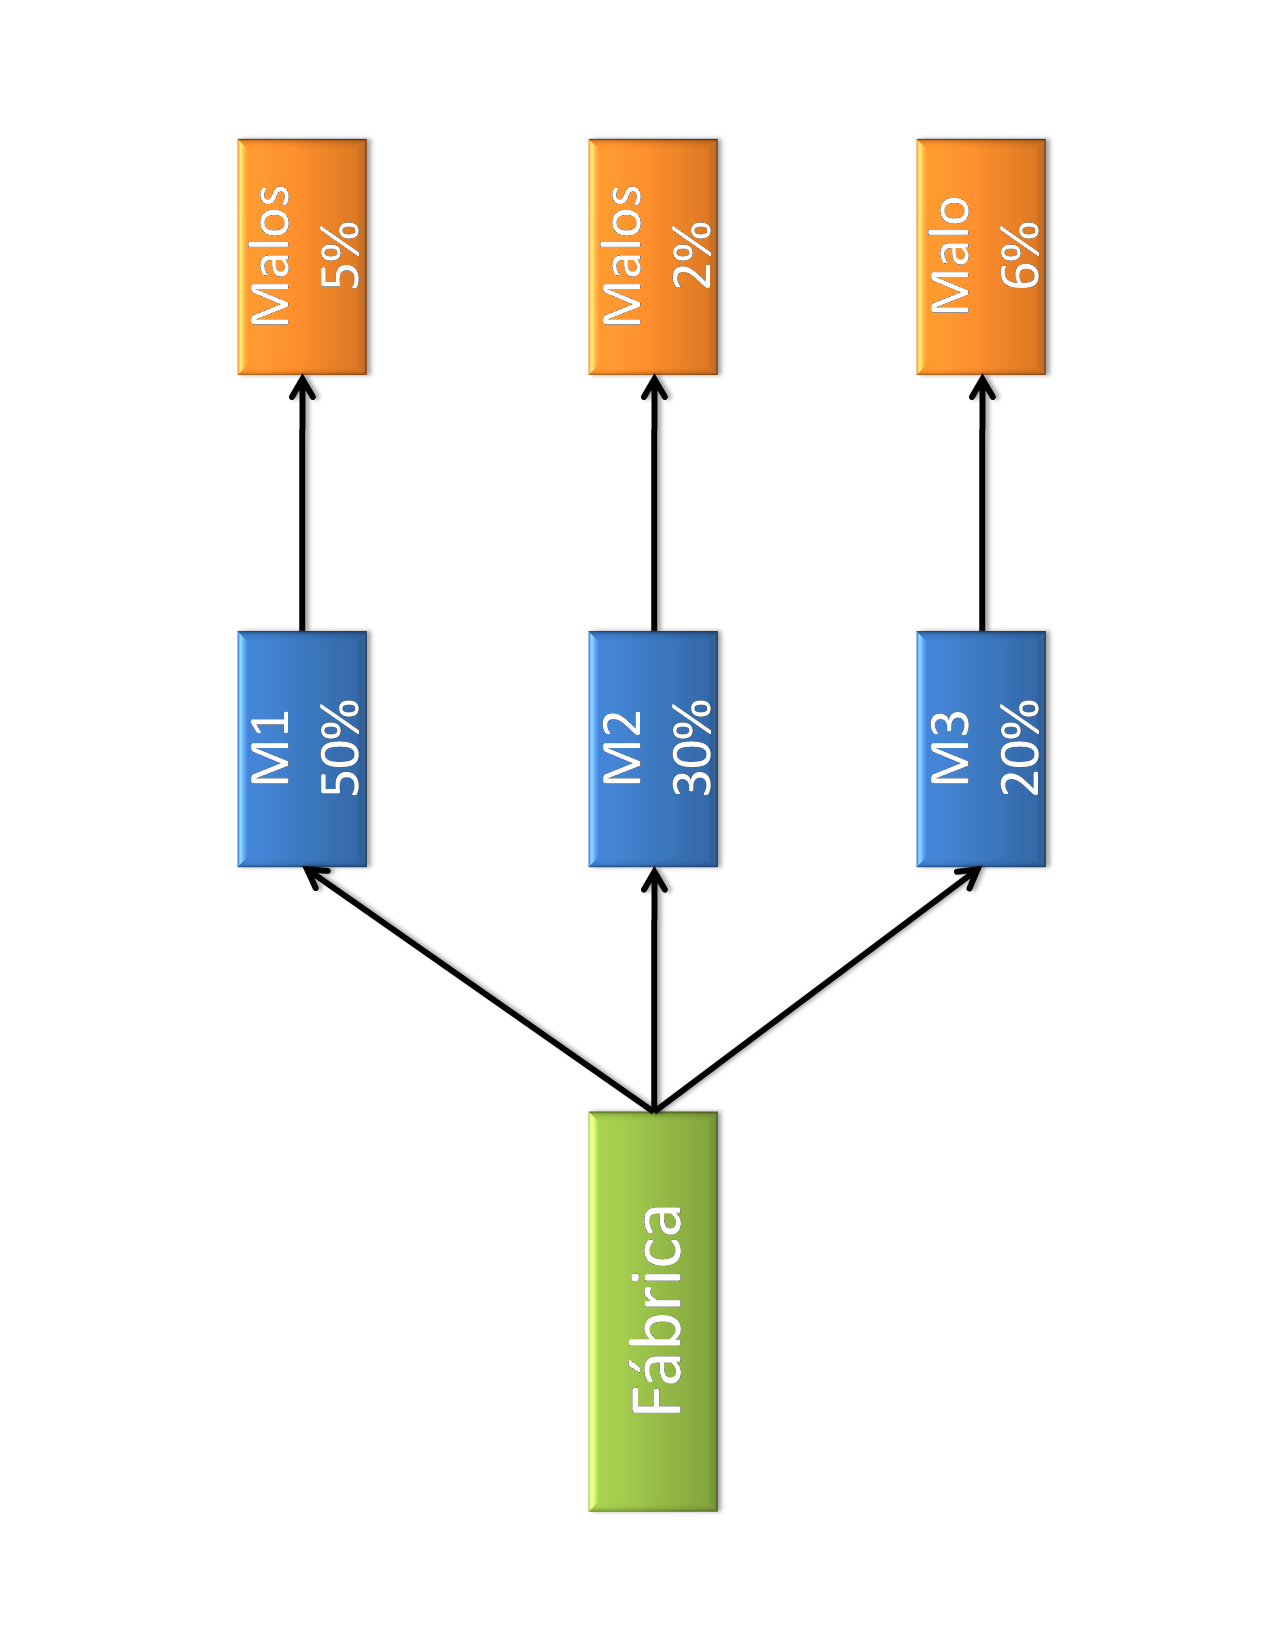
\includegraphics[angle=-90, scale=0.5]{Fabrica1.pdf}
\caption{\emph{Plano del proceso industrial en la fábrica de bolígrafos}}
\end{figure}

Una pregunta natural que surge es acerca de la probabilidad de selección de un artículo defectuoso y para responder a esta pregunta con <<rigurosidad de probabilísta>> es necesario enfocar nuestra atención en los tópicos básicos que dejamos atrás. En primer lugar el experimento en cuestión es la selección de un bolígrafo. Para este experimento, una terna $(\Omega, \mathfrak{F}, P)$ \footnote{$\Omega$ denota el conjunto de todos lo posibles resultados del experimento, $\mathfrak{F}$ denota una $\sigma$-álgebra y $P$ hace referencia ana medida de probabilidad propiamente definida.}, llamada comúnmente espacio de medida o espacio de probabilidad, está dada por
\begin{enumerate}
  \item El espacio muestral: $\Omega=\{\text{defectuoso}, \text{No defectouso}\}$
  \item La $\sigma$-álgebra: $\mathfrak{F}=\{\Omega, \phi, \{\text{Defectuoso}\}, \{\text{No Defectuoso}\}\}$
  \item La función de probabilidad:
  \begin{align*}
  p: \mathfrak{F} &\longrightarrow [0,1]\\
     \Omega &\longrightarrow 1\\
     \phi &\longrightarrow 0\\
     \{Defectuoso\}&\longrightarrow P(D)\\
     \{Defectuoso\}&\longrightarrow 1-P(D)
  \end{align*}
  en donde, acudiendo al teorema de probabilidad total, se define
  \begin{equation*}
  p(D)=p(D \mid M1)P(M1)+p(D \mid M2)P(M2)+p(D \mid M3)P(M3)
  \end{equation*}
\end{enumerate}

Sin embargo, también es posible plantearse otro tipo de preguntas que sirven para calibrar el proceso de producción de artículos defectuosos. Por ejemplo, cabe preguntarse acerca de la probabilidad de que habiendo seleccionado un artículo defectuoso, éste provenga de la primera máquina\footnote{Por supuesto que la pregunta también es válida al indagar por la probabilidad de que habiendo seleccionado un artículo defectuoso, éste provenga de la segunda o tercera máquina.}. En esta ocasión, el experimento ha cambiado y ahora se trata de seleccionar un artículo defectuoso y para responder a tal cuestionamiento, se debe establecer rigurosamente el espacio de probabilidad que puede estar dado por
\begin{enumerate}
  \item El espacio muestral: $\Omega=\{M1, M2, M3 \}$
  \item La $\sigma$-álgebra: $\mathfrak{F}^+=\{\Omega, \phi, \{M1\}, \{M2,M3\}\}$
  \item La función de probabilidad:
  \begin{align*}
  p: \mathfrak{F}^+ &\longrightarrow [0,1]\\
     \Omega &\longrightarrow 1\\
     \phi &\longrightarrow 0\\
     \{M1\}&\longrightarrow p(M1 \mid D)\\
     \{M2,M3\}&\longrightarrow 1-p(M1 \mid D)
  \end{align*}
  en donde, acudiendo a la definición de probabilidad condicional, se define
  \begin{equation*}
  p(M1 \mid D)=\frac{p(D \mid M1)P(M1)}{p(D \mid M1)P(M1)+p(D \mid M2)P(M2)+p(D \mid M3)P(M3)}
  \end{equation*}
\end{enumerate}

La anterior función de probabilidad se conoce con el nombre de regla de probabilidad de Bayes y, aparte de ser el baluarte de la mayoría de investigaciones estadísticas que se plantean hoy en día, ha sido la piedra de tropiezo de muchos investigadores radicales que trataron de estigmatizar este enfoque tildando a sus seguidores de mediocres matemáticos y pobres probabilistas afirmando que la regla de probabilidad de Bayes es sólo un artilugio diseñado para divertirse en el tablero.

Pues bien, la interpretación de la regla de bayes se puede realizar en el sentido de actualización de la estructura probabilística que gobierna el experimento. Y esta actualización tiene mucho sentido práctico cuando se cae en la cuenta de que la vida real está llena de calibradores y que las situaciones generadas son consecuencia de algún cambio estructural. De esta forma, el conocimiento de la probabilidad de que el artículo sea producido por la primera máquina se actualiza al conocer que este artículo particular es defectuoso y de esta manera calibra la estructura aleatoria que existe detrás del contexto de la fábrica de bolígrafos. Aparte de servir para resolver problemas como el anteriormente mencionado, la regla de bayes ha marcado el comienzo de un nuevo enfoque de análisis de datos, no solamente porque hace explícitas las relaciones causales entre los procesos aleatorios, sino también porque facilita la inferencia estadística y la interpretación de los resultados.
\end{Eje}

En el campo de la medicina, también se ha visto un gran número de la aplicación del teorema de Bayes. A continuación se enuncia uno de ellos:

\begin{Eje}
El Grupo de Trabajo de Servicios Preventivos de los Estados Unidos (USPSTF por sus siglas en inglés) hizo unas nuevas y controversiales recomendaciones sobre la detección del cáncer de mama (ver página $http://www.uspreventiveservicestaskforce.org/uspstf/uspsbrca.htm$), dentro de los cuales, no recomienda el examen de la mamografía en mujeres entre 40 y 49 años de edad, afirmando que la práctica bienal de este examen debe ser una decisión individual según el contexto particular de la paciente, mientras que por muchos años, se han dicho a las mujeres que se debe realizar la mamografía una vez cumplidos los 40 años. Por otro lado, USPSTF sí recomienda tal práctica de forma bienal en grupos de mujeres de entre 50 y 74 años de edad, puesto que USPSTF no encontró suficiente evidencia de beneficio o daño adicional en realizar este examen en mujeres mayores que los 74 años. Otra recomendación que hizo USPSTF es no realizar auto exámanes de senos, contrario a las recomendaciones y consejos que da la mayoría de los profesionales y organizaciones de la salud, incluyendo la \emph{Amerian Cancer Society} (ver $http://www.cancer.org/acs/groups/cid/documents/webcontent/003164-pdf.pdf$).

El autor del blog, después de algunas averiguaciones, encontró que 
\begin{itemize}
    \item Los expertos estiman que un 12.3\% de las mujeres desarrollan formas invasivas del cáncer de mama durante la vida.
    \item La probabilidad de que una mujer desarrolle el cáncer de mama entre los 40 y los 49 años de edad es 1 en 69, y esta probabilidad aumenta a medida que envejezca, de tal forma que llega a ser de 1 en 38 en mujeres de entre 50 y 59 años.
    \item El cáncer de mama es más difícil de detectar en mujeres jóvenes puesto que el tejido mamario es más denso y fibroso. Los expertos estiman que la tasa de un falso positivo es de 97.8 por cada 1000 mujeres de 40 y 49 años, y esta tasa disminuye a 86.6 por cada 1000 mujeres entre 50 y 59 años. 
    \item La tasa de un falso negativo es de 1 por cada 1000 mujeres de 40 y 49 años, y es de 1.1 por cada 1000 mujeres entre 50 y 59 años.
\end{itemize}

Resumiendo las anteriores afirmaciones, tenemos las siguientes probabilidades
\begin{table}[!h]
\centering
  \begin{tabular}{|c|c|c|}\hline
  Probabilidad&\multicolumn{2}{|c|}{Edad}\\\cline{2-3}
  &40 - 49 años&50 - 59 años\\\hline
  $p(\text{Cáncer})$&1/69=0.01449&1/38=0.02632\\
  $p(\text{No cáncer})$&68/69=0.9855&37/38=0.97368\\
  $p(\text{Positivo}|\text{ No cáncer})$&0.0978&0.0866\\
  $p(\text{Negativo}|\text{ No cáncer})$&0.9022&0.9134\\
  $p(\text{Negativo}|\text{ Cáncer})$&0.001&0.0011\\
  $p(\text{Positivo}|\text{ Cáncer})$&0.999&0.9989\\\hline
  \end{tabular}
\end{table}

Utilizando la regla de Bayes, se puede calcular las siguientes probabilidades para mujeres de 40 y 49 años: 
\begin{align*}
P(\text{Cáncer}|\text{Positivo})&=\frac{P(\text{Positivo}|\text{Cáncer})P(\text{Cáncer})}{P(\text{Positivo}|\text{Cáncer})P(\text{Cáncer})+P(\text{Positivo}|\text{No cáncer})P(\text{No cáncer})}\\
&=\frac{0.999*0.01449}{0.999*0.01449+0.0978*0.9855}\\
&=0.1305
\end{align*}

\begin{align*}
P(\text{Cáncer}|\text{Negativo})&=\frac{P(\text{Negativo}|\text{Cáncer})P(\text{Cáncer})}{P(\text{Negativo}|\text{Cáncer})P(\text{Cáncer})+P(\text{Negativo}|\text{No cáncer})P(\text{No cáncer})}\\
&=\frac{0.001*0.01449}{0.001*0.01449+0.9022*0.9855}\\
&=0.0000163
\end{align*}

Similarmente, se puede calcular estas dos probabilidades para las mujeres de 50 y 59 años.
\begin{table}[!h]
\centering
  \begin{tabular}{|c|c|c|}\hline
  Probabilidad&\multicolumn{2}{|c|}{Edad}\\\cline{2-3}
  &40 - 49 años&50 - 59 años\\\hline
  $P(\text{Cáncer}|\text{Positivo})$&0.1305985&0.23769\\
  $P(\text{Cáncer}|\text{Negativo})$&0.0000163&0.0000326\\
  $P(\text{No cáncer}|\text{Positivo})$&0.8694223&0.7623123\\
  $P(\text{No cáncer}|\text{Negativo})$&0.9999837&0.9999674\\\hline
  \end{tabular}
\end{table}
Los resultados de la anterior tabla muestran cómo se cambia la probabilidad de tener cancer condicionado en los resultados de la pruebe. Entre estos valores se puede ver que, con un resultado positivo en el examen, la probabilidad de tener efectivamente el cáncer es aproximadamente diez puntos porcentuales más bajo en mujeres de edad de 40 y 49 años, de donde se puede sustentar la recomendación de no efectuar este examen en mujeres de este rango de edad.
\end{Eje}

\section{Inferencia bayesiana}

El enfoque bayesiano, además de especificar un modelo para los datos observados $\mathbf{Y}=(y_1,\ldots,y_n)$ dado un vector de parámetros desconocidos $\btheta=(\theta_1,\ldots,\theta_K)$, usualmente en forma de densidad condicional  $p(\mathbf{Y} \mid \btheta)$, supone que $\btheta$ es aleatorio y que tiene un densidad \emph{previa} $p(\btheta \mid \bEta)$, donde $\bEta$ es un vector de hiper-parámetros. De esta forma, la inferencia concerniente a $\btheta$ se basa en una densidad \emph{posterior} $p(\btheta \mid \mathbf{Y})$.

En términos de estimación, inferencia y predicción, el enfoque Bayesiano supone dos momentos o etapas:

\begin{enumerate}
  \item Antes de la recolección de las datos, en donde el investigador propone, basado en su conocimiento, experiencia o fuentes externas, una distribución de probabilidad \emph{previa} para el parámetro de interés. Con esta distribución es posible calcular estimaciones puntuales y por intervalo con el fin de confirmar que la distribución propuesta se ajusta al problema de estudio. En esta etapa, basados en la distribución \emph{previa}, también es posible hacer predicciones de cantidades observables.
  \item Después de la recolección de los datos. Siguiendo el teorema de Bayes, el investigador actualiza su conocimiento acerca del comportamiento probabilístico del parámetro de interés mediante la distribución \emph{posterior} de este. Con esta distribución es posible calcular estimaciones puntuales y por intervalo justo como en el enfoque frecuentista. En esta etapa, basados en la distribución \emph{posterior}, también es posible hacer predicciones de cantidades observables y pruebas de hipótesis acerca de la adecuación del mejor modelo a los datos observados.
\end{enumerate}

\subsection{Inferencia \emph{previa}}

Con las anteriores expresiones es posible calcular la probabilidad \emph{previa} de que $\btheta$ esté en una determinada región $G$ como
\begin{equation}
Pr(\btheta\in G)=\int_G p(\btheta \mid \bEta)\ d\btheta
\end{equation}

En esta primera etapa también es posible calcular, con fines confirmatorios \cite{Carlin96}, la estimación puntual para el vector $\btheta$ dada por alguna medida de tendencia central para la distribución $p(\btheta \mid \bEta)$. En particular, si se escoge la media, entonces
\begin{equation}\label{est.prio}
\hat{\btheta}=E(\btheta)=\int \btheta \ p(\btheta \mid \bEta)\ d\btheta
\end{equation}

También es posible calcular una región $C$ de $100\times(1-\alpha)\%$ de credibilidad\footnote{La interpretación de las regiones de credibilidad bayesianas difiere de la interpretación de las regiones de confianza frecuentistas. La primera se refiere a la probabilidad de que el verdadero valor de $\btheta$ esté en la región. La segunda se refiere a la región de la distribución muestral para $\btheta$ tal que, dados los datos observados, se podría esperar que el $100\times\alpha\%$ de las futuras estimaciones de $\btheta$ no pertenecieran a dicha región.} para $\btheta$ que en esta primera etapa es tal que
\begin{equation}
1-\alpha \leq Pr(\btheta \in C)=\int_Cp(\btheta \mid \bEta)\ d\btheta
\end{equation}

\subsection{Inferencia \emph{posterior}}
Una vez recolectados los datos, se actualizan las cálculos descritos en la sección anterior. Podemos calcular la probabilidad \emph{posterior} de que $\btheta$ esté en la región $G$ dados los datos observados como
\begin{equation}
Pr(\btheta\in G  \mid \mathbf{Y})=\int_G p(\btheta \mid \mathbf{Y})\ d\btheta
\end{equation}

También es posible calcular la estimación puntual para el vector $\btheta$ dados los datos observados. Ésta está dada por alguna medida de tendencia central para la distribución $p(\btheta \mid \mathbf{Y})$. En particular, si se escoge la media, entonces
\begin{equation}
\hat{\btheta}=E(\btheta \mid \mathbf{Y})=\int \btheta \ p(\btheta \mid \mathbf{Y})\ d\btheta
\end{equation}

La región $C$ de $100\times(1-\alpha)\%$ de credibilidad es tal que
\begin{equation}
1-\alpha \leq Pr(\btheta \in C \mid \mathbf{Y})=\int_Cp(\btheta \mid \mathbf{Y})\ d\btheta
\end{equation}

También la distribución posterior del parámetro $\btheta$ es útil para el procedimiento de juzgamiento de hipótesis en el ámbito del análisis bayesiano. Esto se lleva a cabo por medio del factor de Bayes que se presentará más adelante.

\subsection{Inferencia predictiva}

En términos de inferencia predictiva existen dos etapas que cubren las <<actuales>> suposiciones acerca del vector de parámetros $\btheta$. En una primera etapa - antes de la observación de los datos - la suposición <<actual>> de $\btheta$ está dada por la densidad  \emph{previa} $p(\btheta \mid \bEta)$. En estos términos, utilizando el Resultado \ref{Res131},  la distribución predictiva  \emph{previa} de $\mathbf{Y}$ está dada por
\begin{equation}
p(\mathbf{y})=\int p(\mathbf{Y} \mid \btheta)p(\btheta \mid \bEta)\ d\btheta
\end{equation}

La segunda etapa - después de la recolección de los datos - actualiza las suposiciones acerca de $\btheta$ puesto que ahora éste sigue una distribución \emph{posterior} dada por (\ref{Bayes}). Por lo tanto, la distribución predictiva  \emph{posterior} de $\mathbf{Y}$ está dada por
\begin{align}\label{predictpos}
p(\tilde{\mathbf{y}} \mid \mathbf{Y})&=\int p(\tilde{\mathbf{y}},\btheta \mid \mathbf{y})\ d\btheta \notag \\
&=\int p(\tilde{\mathbf{y}} \mid \btheta,\mathbf{Y})p(\btheta \mid \mathbf{Y})\ d\btheta \notag \\
&=\int p(\tilde{\mathbf{y}} \mid \btheta)p(\btheta \mid \mathbf{Y})\ d\btheta
\end{align}
donde $p(\tilde{\mathbf{y}} \mid \btheta)$ es la distribución de los datos evaluada en los nuevos valores $\tilde{\mathbf{y}}$. La segunda línea de la anterior igualdad se obtiene utilizando el resultado \ref{Res121}  y la última línea se obtiene del resultado \ref{Res122} de la independencia condicional.

\section{Información \emph{previa}}

La escogencia de una distribución previa es muy importante en el análisis bayesiano, puesto que ésta afecta directamente en la distribución posterior, tal como lo ilustra el teorema de Bayes. En primer lugar, la distribución previa debe describir adecuadamente los conocimientos previos sobre los parámetros objetivos de estimación. Por ejemplo, si se cree que un parámetro toma valores cercanos a 10, entonces la distribución escogida para representarla también debe tomar valores cercanos a 10, por ejemplo, una distribución normal centrada en ese valor. Por otro lado, dado que en la literatura existe un gran número de distribuciones, algunas muy similares entre ellas, a la hora de escoger una distribución previa también debe tener en cuenta las implicaciones a la hora de efectuar cálculos de la estimación puntual o de intervalo de crediblidad, procurando en la mayoría de casos, obtener una distribución posterior fácil de manejar. A continuación exponemos algunos aspectos generales relacionados con esta distribución previa.

\subsection{Distribuciones conjugadas}

Como se verá en los capítulos siguientes, muchos problemas de inferencia bayesiana comparten la agradable cualidad de que la forma funcional de la distribución \emph{previa} para el parámetro de interés resulta ser la misma de la distribución \emph{posterior}. Por ejemplo:

\begin{itemize}
  \item Cuando se tiene una muestra aleatoria de variables con distribución Bernoulli de parámetro $\theta$, es factible pensar que una distribución \emph{previa} apropiada para este parámetro es la distribución Beta; bajo este escenario, la distribución \emph{posterior} también resulta ser Beta.
  \item En el caso en que se quiera modelar el parámetro $\theta$ concerniente a una variable aleatoria con distribución Poisson, es posible asignar como candidata para distribución \emph{previa} a la distribución Gamma; en este caso la distribución \emph{posterior} también resulta ser Gamma.
\end{itemize}

Las distribuciones conjugadas son deseadas en el análisis bayesiano pues en primer lugar, la distribución posterior del parámetro $\theta$ es considerada como la actualización del conocimiento acerca de este después de la recolección de los datos, entonces al tener la misma forma funcional que la distribución previa, puede ser comparada a ésta y así ver claramente cómo es la influencia de los datos observados sobre la creencia acerca de $\theta$; en segundo lugar, el hecho de que la distribución posterior sea de la misma forma funcional que la previa permite que la actualización de información se pueda llevar a cabo sistemáticamente, pues cada vez que se observan nuevos datos, la anterior distribución posterior puede ser tomada como la distribución previa y así producir una nueva distribución posterior. 

A continuación exponemos la definición rigurosa de las distribuciones conjungadas y algunos tópicos relacionados.

\begin{Defi}
Sea $\mathcal{F}=\{p(\mathbf{Y} \mid \btheta)\}$ una familia de distribuciones de probabilidad. Una familia de distribuciones $\mathcal{P}$ se dice conjugada con respecto a $\mathcal{F}$ si para toda distribución \emph{previa} $p(\btheta) \in \mathcal{P}$ y para toda distribución de muestreo o verosimilitud de las observaciones $p(\mathbf{Y} \mid \btheta)$, $p(\btheta \mid \mathbf{Y})$ también pertenece a la familia $\mathcal{P}$.
\end{Defi}

Esta definición es en la mayoría de los casos prácticos muy útil. Sin embargo, \citeasnoun{Migon} describe los siguientes dos casos en donde esta definición es completamente inútil:

\begin{enumerate}
\item (Caso amplio) Sea $\mathcal{P}=\{\emph{Todas las distribuciones de probabilidad}\}$ y $\mathcal{F}$ cualquier familia de distribuciones de probabilidad. Entonces $\mathcal{P}$ es conjugada con respecto a $\mathcal{F}$ puesto que toda posible distribución \emph{posterior} será un miembro de $\mathcal{P}$.
\item (Caso restringido) Sea $\mathcal{P}=\{p  \mid  p(\theta=\theta_0)=1\}$, esto es, $\mathcal{P}$ corresponde a todas las distribuciones concentradas en un punto. Sea $\mathcal{F}$ cualquier familia de distribuciones de probabilidad. De esta manera, la distribución \emph{posterior} de $\theta$ estará dada por
    \begin{align*}
    p(\theta \mid Y)\propto
    p(Y \mid \theta)p(\theta)
    &=
    \begin{cases}
    p(Y \mid \theta)\times 1 \ \ \ \ \text{si $\theta=\theta_0$}\\
    p(Y \mid \theta)\times 0 \ \ \ \ \text{si $\theta\neq\theta_0$}\\
    \end{cases}\\
    &=
    \begin{cases}
    p(Y \mid \theta) \ \ \ \ \text{si $\theta=\theta_0$}\\
    0           \ \ \ \ \text{si $\theta\neq\theta_0$}\\
    \end{cases}
    \end{align*}

    De lo anterior y dado que $\int p(\theta \mid Y)\ d\theta=1$, entonces $p(Y \mid \theta)=1$ si y sólo si $\theta=\theta_0$. Con el anterior razonamiento, se concluye que $\mathcal{P}$ es conjugada con respecto a $\mathcal{F}$.
\end{enumerate}

Por lo tanto, se deben buscar distribuciones \emph{previa} que sean conjugadas de una forma tan amplia que permita proponer una distribución \emph{previa} adecuada, pero al mismo tiempo tan restringida para que la definición de conjugada tenga sentido práctico. Ahora introducimos una familia de distribuciones muy importante para el desarrollo de la teoría estadística, tanto en el ámbito bayesiano como en el clásico.

\subsubsection*{Familia exponencial}

Dependiendo de la naturaleza del parámetro $\theta$, la familia exponencial puede ser uniparamétrica o multiparamétrica. En el primer caso, una distribución de probabilidad pertenece a la familia exponencial uniparamétrica si se puede escribir de la forma
\begin{equation}\label{uniexpo}
p(Y \mid \theta)=\exp\{d(\theta)T(y)-c(\theta)\}h(y)
\end{equation}

donde $T(y)$ y $h(y)$ son funciones que dependen de $y$ únicamente, y $d(\theta)$ y $c(\theta)$ son funciones que depende de $\theta$ únicamente. Análogamente, una distribución de probabilidad pertenece a la familia exponencial multi-paramétrica si se puede escribir de la forma
\begin{equation}\label{multiexpo}
p(Y \mid \btheta)=\exp\{\mathbf{d}(\btheta)'\mathbf{T}(y)-c(\btheta)\}h(y)
\end{equation}
donde $\mathbf{T}(y)$ y $\mathbf{d}(\btheta)$ son funciones vectoriales, $h(y)$ y $c(\btheta)$ son funciones reales.

La ventaja de la familia exponencial radica en que es una familia relativamente restringuida de distribuciones y a la vez conserva la propiedad de ser distribuciones conjugadas, tal como muestra el siguiente resultado:

\begin{Res}\label{FE1}
Sea $Y$ una variable aleatoria con función de densidad perteneciente a la familia exponencial uniparamétrica, entonces la familia exponencial uniparamétrica es conjugada con respecto a sí misma.
\end{Res}

\begin{proof}
Observando la expresión (1.5.1), se debe encontrar una distribución \emph{previa} en la familia exponencial uniparamétrica, tal que la distribución \emph{posterior}, resultante del producto de la distribución \emph{previa} con la verosimilitud, sea también miembro de la familia exponencial uniparamétrica. Con base en lo anterior, la distribución \emph{previa}, parametrizada por el hiperparámetro $\alpha$, debe ser una función exponencial de los términos $d(\theta)$ y $c(\theta)$ como lo afirma \citeasnoun{Jordan}. Esto es,
\begin{equation}
p(\theta \mid \alpha)\propto\exp\{w(\alpha) d(\theta)-\delta c(\theta)\},
\end{equation}

donde $\delta$ es una constante real (posiblemente dependiente de $\alpha$). Por otro lado, para garantizar que $p(\theta \mid \alpha)$ sea una auténtica función de densidad se normaliza de la siguiente manera
\begin{equation}
p(\theta \mid \alpha)=\frac{1}{k(\alpha,\delta)}\exp\{w(\alpha) d(\theta)-\delta c(\theta)\},
\end{equation}

con
\begin{equation*}
k(\alpha,\delta)=\int\exp\{w(\alpha) d(\theta)-\delta c(\theta)\} \ d\theta.
\end{equation*}

De esta manera, no es difícil comprobar que la definición de distribución \emph{previa}, parametrizada por el hiper-parámetro $\alpha$, pertenece a la familia exponencial, puesto que
\begin{equation}
p(\theta \mid \alpha)=\exp\{\underbrace{w(\alpha)}_{d(\alpha)} \underbrace{d(\theta)}_{T(\theta)} - \underbrace{\ln k(\alpha,\delta)}_{c(\alpha)}\}\underbrace{\exp\{-\delta c(\theta)\}}_{h(\theta)}.
\end{equation}

Por otro lado, del teorema de Bayes se tiene que
\begin{align*}
p(\theta \mid Y) &\propto p(Y \mid \theta)p(\theta \mid \alpha)\\
&=\exp\{w(\alpha) d(\theta) + d(\theta)T(y) - c(\theta) -\ln k(\alpha,\delta) \}\exp\{-\delta c(\theta)\}h(y)\\
&=\exp\{\underbrace{[\alpha+T(y)]}_{d(y)} \underbrace{d(\theta)}_{T(\theta)} -\underbrace{[\ln k(\alpha,\delta)-\ln h(y)]}_{c(y)}\} \underbrace{\exp\{-(\delta+1) c(\theta)\}}_{h(\theta)}\\
&\propto \exp\{[w(\alpha)+T(y)] d(\theta)\}\exp\{-(\delta+1) c(\theta)\}.
\end{align*}

Por lo tanto, la distribución \emph{posterior} resultante también pertenece a la familia exponencial uniparamétrica.
\end{proof}

La extensión del anterior resultado para el caso cuando tenemos una muestra aleatoria de observaciones es sencilla, tal como se expone a continuación:
\begin{Res}
Sean $\mathbf{Y}=\{Y_1, \ldots, Y_n\}$ una muestra aleatoria de variables distribuidas con función de densidad común perteneciente a la familia exponencial uniparamétrica, cuya función de densidad conjunta $p(\mathbf{Y} \mid \theta)$ también pertenece a la familia exponencial uniparamétrica. Bajo las anteriores condiciones la familia exponencial uniparamétrica es conjugada con respecto a sí misma.
\end{Res}

\begin{proof}
La demostración es inmediata utilizando el resultado anterior y notando que la forma funcional de la densidad conjunta para $\mathbf{Y}$ es
\begin{equation}
p(\mathbf{Y} \mid \theta)=\exp\left\{d(\theta)\sum_{i=1}^nT(y_i)-nc(\theta)\right\}\prod_{i=1}^nh(y_i)
\end{equation}
la cual hace parte de la familia exponencial.
\end{proof}

Otra extensión del resultado \ref{FE1} corresponde al caso cuando la distribución de la observación está reparametrizado por un vector de parámetros $\btheta$. A continuación se expone el resultado y la prueba correspondiente.

\begin{Res}
Sean $Y$ una variable aleatoria con función de densidad perteneciente a la familia exponencial multiparamétrica. Sea $\btheta$ el parámetro de interés con distribución \emph{previa} parametrizada por un vector de hiperparámetros $\bEta$ y perteneciente a la familia exponencial multiparamétrica. Entonces la familia exponencial multiparamétrica es conjugada con respecto a sí misma.
\end{Res}

\begin{proof}
En primer lugar, la distribución de probabilidad de $Y$ perteneciente a la familia exponencial  multiparamétrica está dada por (1.5.2). Siguiendo el mismo razonamiento de la demostración del Resultado 1.5.1, la distribución \emph{previa} del parámetro de interés debe estar definida de la siguiente manera
\begin{equation}
p(\btheta \mid \bEta)=\exp\left\{\underbrace{w(\bEta)'}_{\mathbf{d}(\bEta)}
\underbrace{\mathbf{d}(\btheta)}_{\mathbf{T}(\btheta)} - \underbrace{\ln k(\bEta,\delta)}_{c(\bEta)}\right\}\underbrace{\exp\{-\delta c(\btheta)\}}_{h(\btheta)},
\end{equation}

con
\begin{equation*}
k(\bEta,\delta)=\int\exp\{w(\bEta)'\mathbf{d}(\btheta)-\delta c(\btheta)\} \ d\btheta.
\end{equation*}

Utilizando el teorema de Bayes, se tiene que, la distribución \emph{posterior} del parámetro $\theta$ es
\begin{align*}
p(\btheta \mid Y) &\propto p(Y \mid \btheta)p(\btheta \mid \bEta)\\
&= \exp\{\mathbf{T}(y)'\mathbf{d}(\btheta) - c(\btheta) + w(\bEta)' \mathbf{d}(\btheta) - \delta c(\btheta) - \ln k(\bEta,\delta) +\ln h(y)\}\\
& =
\exp\left\{\underbrace{(w(\bEta)+\mathbf{T}(y))'}_{\mathbf{d}(y)}
\underbrace{\mathbf{d}(\btheta)}_{\mathbf{T}(\theta)} - \underbrace{\left[\ln k(\bEta,\delta)-\ln h(y)\right]}_{c(y)}\right\}\underbrace{\exp\{-(\delta+1)c(\btheta)\}}_{h(\btheta)}
\end{align*}

La anterior expresión también hace parte de la familia exponencial biparamétrica y con esto se concluye la demostración
\end{proof}

Nótese que el anterior resultado también cobija situaciones donde la verosimilitud sea perteneciente a la familia exponencial uniparamétrica. Más aún, a cualquier familia exponencial multiparamétrica de orden menor o igual al orden de la distribución \emph{previa}.

\begin{Res}
Sean $\mathbf{Y}=\{Y_1, \ldots, Y_n\}$ una muestra aleatoria con función de densidad conjunta o verosimilitud dada (1.4.4). Bajo este escenario la familia exponencial multi-paramétrica es conjugada con respecto a sí misma.
\end{Res}

\begin{proof}
La demostración sigue los mismos lineamentos que la demostración del resultado anterior concluyendo que la distribución \emph{posterior} de $\btheta$ está dada por
\begin{align*}
&p(\btheta \mid \mathbf{Y}) \propto p(\mathbf{Y} \mid \btheta)p(\btheta \mid \bEta)\\
&= \exp\left\{\sum_{i=1}^n\mathbf{T}(y_i)'\mathbf{d}(\btheta) - nc(\btheta) + \bEta' \mathbf{d}(\btheta) - \delta c(\btheta) - \ln k(\bEta,\delta) +\sum_{i=1}^n\ln h(y_i)\right\}\\
& =\exp\left\{\underbrace{\left(\bEta+\sum_{i=1}^n\mathbf{T}(y_i)\right)'}_{\mathbf{d}(\mathbf{y})}
\underbrace{\mathbf{d}(\btheta)}_{\mathbf{T}(\theta)} - \underbrace{\left[\ln k(\bEta,\delta)-\sum_{i=1}^n\ln h(y_i)\right]}_{c(\mathbf{y})}\right\} \\
&  \times \underbrace{\exp\left\{-(\delta+n)c(\btheta)\right\}}_{h(\btheta)}
\end{align*}
La anterior expresión también hace parte de la familia exponencial.
\end{proof}

Ahora, estudiamos las expresiones relacionadas con la distribución predictiva de nuevas observaciones dentro del contexto de la familia exponencial:
\begin{Res}
Sea $Y$ una variable aleatoria con función de densidad perteneciente a la familia exponencial, dada por (\ref{uniexpo}). Sea $\theta$ el parámetro de interés con distribución \emph{previa} en la familia exponencial biparamétrica. La distribución predictiva \emph{previa} de $Y$ está dada por
\begin{equation}
p(Y)=\frac{k(\alpha+T(y),\delta+1)}{k(\alpha,\delta)}h(y)
\end{equation}

donde 
\begin{equation*}
k(a,b)=\int \exp\{w(a) d(\theta)-b c(\theta)\}\ d\theta
\end{equation*}
\end{Res}

\begin{proof}
\begin{align*}
p(Y)&=\int p(\theta)p(Y \mid \theta)\ d\theta\\
&=\int \exp\{w(\alpha) d(\theta)-\ln k(\alpha,\delta)-\delta c(\theta)\}\exp\{d(\theta)T(y)-c(\theta)\}h(y)d\theta\\
&=\frac{h(y)}{k(\alpha,\delta)}\int \exp\{[w(\alpha)+T(y)]d(\theta)-(\delta+1)c(\theta)\}d\theta\\
&=\frac{k(\alpha+T(y),\delta+1)h(y)}{k(\alpha,\delta)}
\end{align*}

donde
\begin{equation*}
k(\alpha,\delta)=\int \exp\{w(\alpha) d(\theta)-\delta c(\theta)\}\ d\theta
\end{equation*}

y
\begin{equation*}
k(\alpha+T(y),\delta+1)=\int \exp\{[w(\alpha)+T(y)]d(\theta)-(\delta+1)c(\theta)\} \ d\theta.
\end{equation*}
\end{proof}

La extensión al caso de contar con una muestra aleatoria de observaciones se encuentra a continuación:

\begin{Res}
Sea $\mathbf{Y}=\{Y_1\ldots,Y_n\}$ una muestra aleatoria con función de densidad conjunta perteneciente a la familia exponencial, dada por (1.4.4). Sea $\theta$ el parámetro de interés con distribución \emph{previa} dada por (1.4.5). La distribución predictiva \emph{previa} de $\mathbf{Y}$ está dada por

\begin{equation}
p(\mathbf{Y})=\frac{k(\alpha+T(\mathbf{y}),\delta+n)}{k(\alpha,\beta)}h(\mathbf{y})
\end{equation}
donde $k$ se define tal como en el resultado anterior.
\end{Res}

\begin{proof}
La prueba se tiene de inmediato siguiendo los lineamentos de la demostración del anterior resultado.
\end{proof}

\begin{Res}
En términos de la distribución predictiva \emph{posterior}, se tiene que para una sola observación $\tilde{y}$, ésta está dada por
\begin{equation}
p(\tilde{y} \mid Y)=\frac{k(\alpha+T(y)+T(\tilde{y}),\delta+2)}{k(\alpha+T(y),\delta+1)}h(\tilde{y})
\end{equation}
y en el caso en donde se tiene una muestra aleatoria, entonces la distribución predictiva \emph{posterior} para una nueva muestra $\tilde{\mathbf{y}}=\{\tilde{y}_1,\ldots,\tilde{y}_{n^*}\}$ de tamaño $n^*$ está dada por
\begin{equation}
p(\tilde{\mathbf{y}} \mid \mathbf{Y})=
\frac{k(\alpha+T(\mathbf{y})+T(\tilde{\mathbf{y}}),\delta+n+n^*)}
{k(\alpha+T(\mathbf{y}),\delta+n)}h(\tilde{\mathbf{y}})
\end{equation}
\end{Res}

\begin{proof}
De la definición de distribución predictiva \emph{posterior} dada por la expresión (\ref{predictpos}) se tiene que
\begin{align*}
p(\tilde{y} \mid Y)&=\int p(\tilde{y} \mid \theta)p(\theta \mid y)\ d\theta\\
&=\int \exp\{d(\theta)T(\tilde{y})-c(\theta)\}h(\tilde{y})\dfrac{\exp\{[w(\alpha)+T(y)]d(\theta)-(\delta+1)c(\theta)\}}{k(\alpha+T(y),\delta+1)}\ d\theta\\
&=\frac{h(\tilde{y})}{k(w(\alpha)+T(y),\delta+1)}\int \exp\{[\alpha+T(y)+T(\tilde{y})]d(\theta)-(\delta+2)c(\theta)\}\ d\theta\\
&=\frac{k(\alpha+T(y)+T(\tilde{y}),\delta+2)}{k(\alpha+T(y),\delta+1)}h(\tilde{y}),
\end{align*}

con
\begin{equation*}
k(\alpha+T(y)+T(\tilde{y}),\delta+2)=\int \exp\{[w(\alpha)+T(y)+T(\tilde{y})]d(\theta)-(\delta+2)c(\theta)\}\ d\theta.
\end{equation*}

La demostración para la nueva muestra se lleva a cabo de manera análoga.
\end{proof}

\subsection{Distribuciones \emph{previa} no informativas}

Cuando no existe una base poblacional sobre el parámetro de interés o cuando existe total ignorancia de parte del investigador acerca del comportamiento de probabilístico del parámetro, es necesario definir distribuciones \emph{previa} que sean no informativas. Es decir, definir distribuciones \emph{previa} que jueguen un papel mínimo en términos de influencia en la distribución \emph{posterior}. Una característica de estas distribuciones es que su forma es vaga, plana o difusa, cumpliendo así el objetivo de no influenciar a la distribución \emph{posterior}. Por tanto la pregunta de interés que surge en este instante es: ¿cómo seleccionar distribuciones \emph{previa} no informativas\footnote{Existen muchas denominaciones para las distribuciones uniformes que no son informativas. Por ejemplo, Box Tiao proponen el nombre de distribuciones localmente uniformes para asegurar que cumplan con las condiciones de función de densidad de probabilidad en un rango particular del espacio paramétrico. Sin embargo, en este texto vamos a utilizar la expresión <<no informativa>> al referirse a este tipo de distribuciones a previa.} sobre el parámetro de interés?

En los anteriores términos, la distribución uniforme define una distribución \emph{previa} que cumple con las características de no información en la mayoría de escenarios. Específicamente en aquellos problemas en donde el parámetro de interés está limitado a un espacio de muestreo acotado. Por ejemplo, en la distribución Binomial, el parámetro de interés está limitado al espacio de muestreo $[0,1]$. Sin embargo, no en todos los problemas encaja la distribución uniforme. Nótese, por ejemplo, que en el caso en que la distribución exponencial se acomode a los datos como candidata a verosimilitud, entonces el espacio de muestreo del parámetro de interés estaría dado por $(0,\infty)$ en cuyo caso la distribución uniforme no sería conveniente puesto que sería una distribución impropia en el espacio de muestreo del parámetro de interés. Es decir
\begin{equation*}
\text{si } p(\theta)\propto kI_{\Theta}(\theta) \text{, entonces } \int_{\Theta}p(\theta) \ d(\theta)\longrightarrow \infty.
\end{equation*}

donde $\Theta$ denota espacio de muestreo del parámetro $\theta$ y $I$ denota la función indicadora. Por otro lado, una característica importante que debe tener una distribución \emph{previa} no informativa es que sea invariante en términos de transformaciones matemáticas. Es decir, si el parámetro de interés es $\theta$ con distribución \emph{previa} no informativa dada por $p(\theta)$, y sea $\phi=h(\theta)$ una transformaición de $\theta$ por medio de la función $h$, entonces la distribución \emph{previa} de $\phi$ también debería ser no informativa. Sin embargo, la teoría de probabilidad afirma que la distribución de probabilidad de una transformación está dada por
\begin{equation}\label{teo_transf}
p(\phi)=p(\theta) \mid \frac{d\theta}{d\phi} \mid =p(\theta) \mid h'(\theta) \mid ^{-1}
\end{equation}

y claramente si la función $h$ no es una función lineal, entonces los resultados encontrados por medio de este enfoque indicarían que la distribución \emph{previa} $p(\phi)$ sería informativa contradiciendo los supuestos de $p(\theta)$. El siguiente ejemplo ilustra este planteamiento:

\begin{Eje}
Suponga que el parámetro de interés es $\theta$ y que está restringido a un espacio de muestreo dado por el intervalo $[0,1]$. Si se supone completa ignorancia acerca del comportamiento del parámetro, entonces una buena opción, con respecto a la distribución \emph{previa}, sería la distribución uniforme en el intervalo $[0,1]$. Es decir, la distribución \emph{previa} no informativa estaría dada por
\begin{equation*}
p(\theta) = I_{[0,1]}(\theta)
\end{equation*}

Suponga ahora que existe una transformación del parámetro de interés dada por $\phi=h(\theta)=\ln(\theta)$. Por tanto, siguiendo (\ref{teo_transf}) se tiene que la distribución de $\phi$ está dada por
\begin{equation*}
p(\phi)=I_{(-\infty,0)}(\phi)e^{\phi}
\end{equation*}

la cual es informativa con respecto al parámetro $\phi$. Sin embargo, es el mismo problema y existe una contradicción en términos de que para $\theta$ se desconoce todo, pero para una función $\phi$ existe evidencia de que el parámetro se comporta de cierta manera.
\end{Eje}

Para palear las anteriores diferencias, es necesario encontrar una distribución \emph{previa} no informativa que sea invariante a transformaciones matemáticas. La distribución \emph{previa} no informativa de Jeffreys, definida a continuación, cuenta con esta agradable propiedad.

\begin{Defi}
Si la verosimilitud de los datos está determinada por un único parámetro $\theta$, la distribución \emph{previa} no informativa de Jeffreys tiene distribución de probabilidad dada por
\begin{equation}
p(\theta)\propto (I(\theta))^{1/2}
\end{equation}

con $I(\theta)$ la información de Fisher definida como
\begin{align*}
I(\theta)&=E\left\{\left[\frac{\partial}{\partial\theta}\log{p(\mathbf{Y}\mid\theta)}\right]^2\right\}\\
&=-E\left\{\dfrac{\partial^2}{\partial\theta^2}\log{p(\mathbf{Y}\mid\theta)}\right\}
\end{align*}

Si la verosimilitud de los datos está determinada por un vector de parámetros $\btheta$, la distribución \emph{previa} no informativa de Jeffreys tiene distribución de probabilidad dada por
\begin{equation}
p(\theta)\propto |\mathbf{I}(\btheta)|^{1/2}
\end{equation}

donde $\mathbf{I}$ es la matriz de información de Fisher, cuyo elemento en la fila $i$ y columna $j$ está definida como
\begin{align*}
\mathbf{I}_{[ij]}(\btheta)&=E\left\{\left[\frac{\partial}{\partial\theta_i}\log{p(\mathbf{Y}\mid\theta)}\right]\left[\frac{\partial}{\partial\theta_j}\log{p(\mathbf{Y}\mid\btheta)}\right]\right\}\\
&=-E\left\{\dfrac{\partial^2}{\partial\theta_i\partial\theta_j}\log{p(\mathbf{Y}\mid\btheta)}\right\}
\end{align*}
donde $\theta_i$ y $\theta_j$ son los elementos $i$ y $j$ del vector $\btheta$.
\end{Defi}

Nótese que si la verosimilitud de las observaciones pertenecen a la familia de distribuciones exponencial, entonces la distribución previa de Jeffreys no es difícil de calcular. Por otro lado nótese que la distribución previa no informativa de Jeffreys depende, de cierta manera, del mecanismo probabilístico que rige a los datos. Lo anterior hace que ciertos críticos de la estadística bayesiana critiquen este enfoque puesto que se supone que la formulación de la distribución a previa es independiente de los datos observados.

A continuación se evidencia la propiedad de esta distribución previa de seguir siendo no informativa con diferentes parametrizaciones. 
\begin{Res}
La distribución \emph{previa} no informativa de Jeffreys es invariante a transformaciones uno a uno. Es decir, si $\phi=h(\theta)$, entonces $p(\phi)\propto(I(\phi))^{1/2}$.
\end{Res}

\begin{proof}
En primer lugar nótese que
\begin{align*}
I(\theta)=\mathbf{J}(\phi) \mid \frac{\partial\phi}{\partial\theta} \mid ^{2}
\end{align*}

puesto que al utilizar la regla de la cadena del cálculo matemático se tiene que
\begin{align*}
\mathbf{J}(\phi)= - E\left[\frac{\partial^2 \log p(\mathbf{Y} \mid \phi)}{\partial\phi^2}\right]
&= - E\left[\frac{\partial}{\partial\phi}\left(\frac{\partial \log p(\mathbf{Y} \mid \phi)}{\partial\phi}\right)\right]\\
&= - E\left[\frac{\partial}{\partial\theta}\left(\frac{\partial \log p(\mathbf{Y} \mid \phi)}{\partial\phi}\right) \mid \frac{\partial\theta}{\partial\phi} \mid \right]\\
&= - E\left[\frac{\partial^2 \log p(\mathbf{Y} \mid \phi)}{d\theta^2} \mid \frac{\partial\theta}{\partial\phi} \mid ^{2}\right]\\
&= - E\left[\frac{\partial^2 \log p(\mathbf{Y} \mid \theta =h^{-1}(\phi))}{d\theta^2} \mid \frac{\partial\theta}{\partial\phi} \mid ^{2}\right]\\
&= I(\theta) \mid \frac{\partial\theta}{\partial\phi} \mid ^{2}
\end{align*}

Ahora, de la definición de función de distribución para una función y utilizando (1.4.11), se tiene que
\begin{align*}
p(\phi)&=p(\theta) \mid \frac{\partial\theta}{\partial\phi} \mid
\propto (I(\theta))^{1/2} \mid \frac{\partial\theta}{\partial\phi} \mid
\propto I(\phi)^{1/2} \mid \frac{\partial\phi}{\partial\theta} \mid  \mid \frac{d\theta}{\partial\phi} \mid =I(\phi)^{1/2}
\end{align*}
\end{proof}

En \citeasnoun[p. 59]{BoxTiao} citan una Tabla de resumen en donde se encuentran distribuciones a previa no informativas para las distribuciones probabilísticas más comunes. A continuación se exponen algunos ejemplos que utilizan este enfoque.

\begin{Eje}
Si $Y$ es una variable aleatoria con distribución Binomial, entonces el espacio de muestreo del parámetro de interés será el intervalo $[0,1]$; sería conveniente utilizar la función de distribución uniforme sobre este intervalo como distribución \emph{previa} no informativa. Con el enfoque de Jeffreys se llega a este mismo resultado puesto que: la información de Fisher para la distribución binomial es $J(\theta)=n/\theta(1- \theta)$ dado que
\begin{equation*}
\log p(Y \mid \theta)=\log \binom{n}{y} + y\log(\theta)+(n-y)\log(1-\theta)
\end{equation*}
y
\begin{equation*}
\frac{\partial^2 \log p(Y \mid \theta)}{\partial\theta^2}=-\frac{y}{\theta^2}-\frac{n-y}{(1-\theta)^2}
\end{equation*}
Por lo tanto al calcular la esperanza, y por consiguiente la información de Fisher, se tiene que
\begin{equation*}
I(\theta)=- E\left[\frac{d^2 \log p(Y \mid \theta)}{d\theta^2}\right]
=\frac{n\theta}{\theta^2}+\frac{n-n\theta}{(1-\theta)^2}= \frac{n}{\theta(1-\theta)}
\end{equation*}
Es decir, la distribución \emph{previa} no informativa para el parámetro de interés $\theta$ es proporcional a $\theta^{-1/2}(1-\theta)^{-1/2}$, la cual comparte la misma forma estructural de una distribución $Beta(1/2,1/2)$ que a su vez es idéntica a la distribución uniforme.  En términos de la distribución \emph{posterior} para el parámetro de interés, se tiene que
\begin{align*}
p(\theta \mid Y) &\propto p(Y \mid \theta) p(\theta)\\
&\propto \theta^{y}(1-\theta)^{n-y}\theta^{-1/2}(1-\theta)^{-1/2}\\
&=\theta^{y+1/2-1}(1-\theta)^{n-y+1/2-1}
\end{align*}
Por tanto, la distribución de $\theta \mid Y$ es $Beta(y+1/2,n-y+1/2)$. Por construcción, esta distribución no está alterada ni influenciada por la distribución \emph{previa} pues la misma es no informativa.
\end{Eje}

\begin{Eje}
\label{EjemPoisson}
Si $\mathbf{Y}=\{Y_1,\ldots,Y_n\}$ es una muestra aleatoria de variables con distribución de Poisson, entonces el espacio de muestreo del parámetro de interés será el intervalo $(0,\infty)$; por tanto utilizar la distribución uniforme como distribución \emph{previa} no informativa no es conveniente. Ahora, la información de Fisher para la distribución conjunta es $I(\theta)=n/\theta$ puesto que
\begin{equation*}
\log p(\mathbf{Y} \mid \theta)=-n\theta+\log(\theta)\sum_{i=1}^ny_i-\sum_{i=1}^n\log(y_i!)
\end{equation*}
y
\begin{equation*}
\frac{\partial^2 \log p(\mathbf{Y} \mid \theta)}{\partial\theta^2}=-\frac{\sum_{i=1}^ny_i}{\theta^2}
\end{equation*}
Por lo tanto al calcular la esperanza, y por consiguiente la información de Fisher, se tiene que
\begin{equation*}
I(\theta)=- E\left[\frac{\partial^2 \log p(\mathbf{Y} \mid \theta)}{\partial\theta^2}\right]
=\frac{\sum_{i=1}^nE(y_i)}{\theta^2}=\frac{n}{\theta}
\end{equation*}
Es decir, la distribución \emph{previa} no informativa para el parámetro de interés es proporcional a $\theta^{-1/2}$. En términos de la distribución \emph{posterior} para el parámetro de interés, se tiene que
\begin{align*}
p(\theta \mid Y) \propto p(Y \mid \theta) p(\theta) \propto e^{-n\theta} \theta^{\sum_{i=1}^ny_i}\theta^{-1/2}
=e^{-n\theta} \theta^{\sum_{i=1}^ny_i-1/2}
\end{align*}
Por tanto, la distribución de $\theta \mid \mathbf{Y}$ es $Gamma(\sum_{i=1}^ny_i+1/2,n)$. Por construcción, esta distribución no está alterada ni influenciada por la distribución \emph{previa} pues la misma es no informativa.
\end{Eje}

\begin{Eje}
Suponga que $\mathbf{Y}=\{Y_1\ldots, Y_n\}$ es una muestra aleatoria con distribución normal de parámetros $(\theta, \sigma^2)'$. Se puede verificar que la matriz de información de Fisher para el vector de parámetros está dada por
\begin{equation}
\begin{pmatrix}
  \frac{n}{\sigma^2} & 0 \\
  0 & \frac{n}{2\sigma^4} \\
\end{pmatrix}
\end{equation}

cuyo determinante está dado por $\frac{n^2}{2\sigma^6}$. Por lo tanto, la distribución a previa no informativa de Jeffreys está dada por
\begin{equation}
p(\theta,\sigma^2)\propto 1/\sigma^3
\end{equation}
\end{Eje}

\section{Pruebas de hipótesis}

A excepción del juzgamiento de hipótesis, las inferencias que hacen los estadísticos bayesianos, acerca de poblaciones normales, son muy similares a las que los estadísticos de la tradición frecuentista, de Neyman y Pearson, hacen.
Consideremos la siguiente situación. Un instrumento mide la posición de un objeto con un determinado error. Éste error está distribuido de manera uniforme en el intervalo (-1cm, 1cm). Supongamos que el instrumento midió la posición de un objeto en +0.9999cm del origen. Planteamos la siguiente hipótesis nula, H: La posición real del objeto es exactamente el origen. Imagine que planteamos este problema de inferencia estadística a los profesores López (frecuentista clásico) y Cepeda (acérrimo bayesiano).
Razonamiento del frecuentista: Si la hipótesis nula es verdadera, ha ocurrido un evento con una probabilidad (a dos colas) de ocurrencia de 0.0001 o menos. Mediante un criterio razonable (nivel de significación), este es un evento muy raro y por lo tanto rechaza H.
Razonamiento del bayesiano: El bayesiano ve las cosas desde un punto de vista diferente. Dada una observación, la verosimilitud asociada con la posición del objeto en el intervalo -0.0001 y +1.9999 es la misma, 0.5. Fuera de esos límites la verosimilitud es nula. Ahora, el origen está dentro de la región en donde la verosimilitud es máxima; por lo tanto sea cual sea la distribución a previa asociada al parámetro de posición, la distribución a posterior tomara el valor cero en cualquier lugar fuera del intervalo -0.0001 y +1.9999. Así, con la observación disponible, no hay evidencia para el rechazo de H.
Bajo esta paradoja, Brewer (2002) sugiere que ambos estadísticos tienen razón, pero a la vez están equivocados. El frecuentista tiene razón en afirmar que, con la evidencia disponible, ha ocurrido un evento extraordinariamente extraño o que la hipótesis nula es falsa. El bayesiano tiene razón en argumentar que, en términos de la situación, no hay evidencia en contra de la hipótesis nula.
Esta paradoja se presenta porque los bayesianos tienden a trabajar dentro de la situación que ellos creen que existe (o al menos creen que ellos creen que existe) y la lógica bayesiana se mueve en ese marco de referencia. Los bayesianos hacen las inferencias en términos de la verosimilitud de los eventos observados, mientras que los frecuentistas hacen inferencias en términos de eventos que ni siquiera han ocurrido. .

\subsection{Factor de Bayes}
El juzgamiento de hipótesis del enfoque frecuentista se puede efectuar en el ámbito Bayesiano por medio del \emph{Factor de Bayes}. Suponiendo que existen dos modelos $M1$ y $M2$ candidatos para $\mathbf{Y}$, se define el \emph{Factor de Bayes} en favor del modelo $M1$ como la razón de las densidades marginales de los datos para los dos modelos y es posible demostrar que es equivale a la siguiente expresión
\begin{equation}\label{FB}
FB=\frac{p(\mathbf{Y} \mid M1)}{p(\mathbf{Y} \mid M2)}=\frac{Pr(M1 \mid \mathbf{Y})/Pr(M2 \mid \mathbf{Y})}{Pr(M1)/Pr(M2)}
\end{equation}

Para evaluar esta última expresión es necesario recurrir a la densidad previa y posterior del parámetro de interés, asumiendo que los modelos están parametrizados por éstos. Se puede ver que cuando los modelos $M1$ y $M2$ tienen la misma distribución previa, entonces el factor de Bayes se reduce a la razón de densidad posterior de los dos modelos. Adicionalmente este factor sólo está definido cuando la integral de la densidad marginal de $\mathbf{Y}$ bajo cada modelo converge. En la expresión (\ref{FB}) se claro que valores grandes del factor muestra evidencias a favor del modelo $M1$, valores menores de 1 a favor del modelo $M2$, mientras que valores cercanos a 1 no muestra evidencias claras hacia ninguno de los dos modelos.

En \citeasnoun{Gelman95} presenta el siguiente ejemplo sencillo sobre la presencia o ausencia de la enfermedad hemofilia, una enfermedad genética especialmente grave las mujeres. Para una mujer quien tiene un hermano portador del gen, el parámetro $\theta$ describe la presencia o ausencia del gen en ella, y toma valores de 1 (presencia del gen) y 0 (ausencia del gen). La distribución previa del parámetro es $P(\theta=1)=P(\theta=0)=0.5$. El objetivo es evaluar el sistema $M_1:\ \theta=1$ y $M_2:\ \theta=0$ con base en el hecho de que ella tiene dos hijos ambos no portadores del gen. De esta forma
\begin{equation*}
FB=\frac{p(y_1=0,\ y_2=0|\theta=1)}{p(y_1=0,\ y_2=0|\theta=0)}=\frac{0.25}{1}=0.25
\end{equation*}
De donde se evidencia mayor apoyo a la hipótesis $\theta=0$.

\subsection{Valor $p$ Bayesiano}
En la inferencia clásica, se define el valor $p$ como la probabilidad de que la estadística de prueba tome valores más extremos a los observados, y se compara con el nivel de significancia, previamente establecidad, para tomar decisión acerca de una hipótesis nula. En el ámbito Bayesiano, el valor $p$ se define como la probabilidad de que la estadística de prueba $T$ calculado sobre los datos replicados $y^{rep}$ sean más extremos al observado, y la probabilidad se toma sobre la distribución posterior del parámetro $\theta$ y la distribución predictiva posterior de $y^{rep}$. Específicamente, queda determinado por
\begin{equation*}
p_B=\int\int_{{T(y^{rep})\geq T(y)}}p(y^{rep}|\theta)p(\theta|y)dy^{rep}d\theta
\end{equation*}

A diferencia del valor $p$ clásico donde solo valores pequeños muestran evidencia en contra de la hipótesis nula, un valor $p$ Bayesiano extremo (menor a 0.01 o mayor a 0.99) sugiere que los valores observados difícilmente pueden ser replicadso si el modelo fuera verdadero.
\section{Criterios de información}

Los criterios de información constituyen una herramienta muy importante en el modelamiento estadístico, pues contribuye a la selección de modelos de manera simple. Existen una variedad de estos criterios, a continuación se describen los dos criterios más comunes en el análisis bayesiano.

\subsubsection*{Criterio DIC}

El criterio de información de devianza (denotada por DIC por los iniciales en inglés) es una generalización del popular criterio AIC para los modelos jerárquicos, y se basa en el concepto de la devianza que se define como
\begin{equation}
D(y, \btheta)=-2*\log(p(y|\btheta))
\end{equation}

cuya media posterior es una medida usual del ajuste del modelo. \citeasnoun{Dempster74} sugirió graficar la distribución posteriori de la devianza para observar el ajuste del modelo a los datos. Una estimación de esta media posterior se basa en simulación de $M$ valores $\btheta^1,\cdots,\btheta^M$ de la distribución posterior de $\btheta$, y está dada por
\begin{equation*}
\hat{E}_D=\frac{1}{M}\sum_{m=1}^MD(y,\btheta^m)
\end{equation*}

El DIC se define como
\begin{equation*}
DIC=\hat{E}_D+p_D
\end{equation*}

Donde $p_D$ es el número efectivo de parámetros. Nótese que en la anterior formulación, el DIC se puede descomponer en dos partes: la parte de la bondad de ajuste del modelo, medido a través de $E_D$,  y la parte que mide la complejidad del modelo $p_D$. Otra formulación equivalente del DIC se obtiene teniendo en cuenta que
\begin{equation*}
p_D=\hat{E}_D - \hat{D}
\end{equation*}

Donde $\hat{D}=-2*\log(p(y|\hat{\btheta}))$ con $\hat{\btheta}$ denotando la media posterior de $\btheta$; es decir, $\hat{D}$ es la estimación de la devianza usando $\hat{\btheta}$, y $p_D$ se puede ver como la media posterior de la devianza menos la devianza de las medias posterior \cite{Spiegel}. De esta forma, el DIC también se puede escribir como
\begin{equation*}
DIC=\hat{D}+2p_D
\end{equation*}

Interpretación de DIC: El modelo con el menor DIC es considerado como el modelo que mejor predice un conjunto de datos con la misma estructura que los datos observados. Al respecto se deben tener en cuenta las siguientes consideraciones:

\begin{itemize}
  \item El DIC puede ser negativo puesto que $p(y|\theta)$ puede tomar valores mayores a 1 asociado a una devianza pequeña.
  \item $p_D$, y por consiguiente DIC, no es invariante a parametrizaciones del modelo. Se sugiere en la práctica usar parametrizaciones que conducen a la normalidad en la distribución posterior.
\end{itemize}

\subsubsection*{Criterio AIC y BIC}

El criterio de información de Akaike (AIC) fue formalmente presentado en \citeasnoun{Akaike}. Este criterio mide la pérdida de información al ajustar un modelo a un conjunto de datos; por esto, se buscan modelos que arrojen valores pequeños de AIC. Posteriormente \citeasnoun{AICc} introdujo el factor de corrección para evitar que el AIC escoja modelos con demasiados parámetros en situaciones de tamaño de muestra pequeño. Por otro lado, el criterio de información bayesiano BIC, también conocido como el criterio de Schwarz \cite{Schwarz}, también está formulado en términos de la función de verosimilitudel modelo y del número de parámetros. La expresión de estos criterios es como sigue:
\begin{align*}
AIC&=-2\log(p(y|\hat{\btheta}))+2p\\
AIC_c&=AIC+\frac{2p^2+2p}{n-p-1}\\
BIC&=-2\log(p(y|\hat{\btheta}))+p\log(n)
\end{align*}

Donde $p$ es el número de parámetros en el modelo y $n$ el número de datos observados. Cabe resaltar que en el criterio BIC hay una mayor penalización por el número excesivo de parámetros que en el criterio AIC, y en la práctica se prefieren los modelos con un BIC menor.

\textbf{Nota:} Se debe recalcar que los dos criterios tienen diferentes enfoques, el criterio BIC se enfoca en identificar el modelo verdadero, mientras que el criterio DIC enfoca en encontrar el modelo con mejor capacidad de predicción.


\section{Acerca de la notación}

Antes de empezar las próximas secciones, es necesario revisar la notación que se seguirá de ahora en adelante. Del teorema de Bayes resultan tres grandes definiciones que constituyen la base de la estadística Bayesiana y que a lo largo de este texto se mencionarán diferenciándolas por medio de la notación. El símbolo más importante de la estadística matemática es $p$, el cual indica que existe una distribución de probabilidad para los datos, para el vector de parámetros, condicional o no. De hecho todos las definiciones y resultados anteriores han estado supeditadas al uso de esta monótona notación. En el ámbito de la notación de investigación internacional es común diferenciar las distribuciones con el fin de hacer más ameno el estudio del enfoque Bayesiano. En este texto se seguirá esta distinción. Un ejemplo claro en donde $ p$ representa cuatro funciones distintas en una sola ecuación es el siguiente:

$$ p(\theta \mid y)=p(y \mid \theta)\frac{p(\theta)}{p(y)}$$

\citeasnoun{Gelman95} explica por qué la notación simple, con el uso (a veces abuso) de la letra $p$ es más rigurosa de lo que, a simple vista, pueda parecer y comenta que,

\begin{quote}
En realidad no me gusta la notación que la mayoría de los estadísticos usan:$f$, para distribuciones de muestreo; $ \pi$, para distribuciones a previa y $ L$, para verosimilitudes. Este estilo de notación se desvía de lo que realmente es importante. La notación no debería depender del orden en que las distribuciones son especificadas. Todas ellas son distribuciones de probabilidad, eso es lo realmente importante.
\end{quote}

Esto tiene sentido, aún más cuando se estudian las propiedades estadísticas de los estimadores desde el punto de vista de la teoría de la medida. Siendo así, el símbolo $p$ se refiere a una notación para una medida de probabilidad, quizás inducida por un elemento aleatorio. De hecho, en la ecuación que determina la regla de Bayes, cada una de las $p$ son medidas de probabilidad que no comparten el mismo espacio de medida (ni la misma $ \sigma$-álgebra, ni el mimo espacio muestral ).

De hecho, todo queda claro al realizar un diagrama que permita ver el espacio de salida y el espacio de llegada de los elementos aleatorios que inducen (si es el caso), cada una de las distribuciones de probabilidad. Por otra parte, Bob Carpenter, concluye que

\begin{quote}
[Una vez resuelto el problema de identificación de los espacios] la notación estadística depende en gran manera del contexto y aunque la regla de Bayes no necesite de mucha explicación, es necesario conocerlo todo acerca del contexto para poder interpretar las funciones que la conforman... El problema se hace mucho más agudo para los estadísticos novatos, pero eso se resuelve con la práctica. Una vez que uno sabe lo que está haciendo, se vuelve obvia la referencia de la distribución $ p$.
\end{quote}

Por lo anterior, es natural que algunos de los textos clásicos de estadística matemática, parezcan olvidar el contexto de las diferentes medidas de probabilidad. En realidad no es que lo olviden, lo que pasa es que los autores no son novatos y asumen que el lector sigue la idea de la referencia de la $ p$ en cuestión. Sin embargo, y lo digo por mi y sólo por mí, sería mejor que no asumieran esa idea. De esta manera, el estudio de estos textos sería un poco menos denso.




